\documentclass[times, twoside, watermark]{zHenriquesLab-StyleBioRxiv}
\usepackage{blindtext}
\usepackage{amsmath}
\pdfoptionalwaysusepdfpagebox=5

% Please give the surname of the lead author for the running footer
\leadauthor{Denovellis} 

\begin{document}

\title{Categorizing the trajectory dynamics of replay}
\shorttitle{Replay Dynamics}

% Use letters for affiliations, numbers to show equal authorship (if applicable) and to indicate the corresponding author
\author[1,\Letter]{Eric L. Denovellis}
\author[2, 3]{Anna K. Gillespie}
\author[2, 3]{Michael E. Coulter}
\author[2, 3, 4]{Loren M. Frank}
\author[1]{Uri T. Eden}

\affil[1]{Department of Mathematics and Statistics, Boston University, Boston, Massachusetts}
\affil[2]{Department of Physiology, University of California, San Francisco, San Francisco, California}
\affil[3]{Kavli Institute for Fundamental Neuroscience, University of California, San Francisco, San Francisco, California}
\affil[4]{Howard Hughes Medical Institute, University of California, San Francisco, San Francisco, California}

\maketitle

%TC:break Abstract
%the command above serves to have a word count for the abstract
\begin{abstract}
During sleep and immobility, hippocampal place cells fire in sequences consistent with temporally compressed versions of trajectories previously run by the animal. These replayed sequences are hypothesized to be an important mechanism for the retrieval of spatial memory in service of consolidation and decision-making. Replay events are typically evaluated based on whether they activate sequences of place cells that represent spatially continuous trajectories through the environment, but recent work has shown that these events can have more complex dynamics. For example, sequences can alternate between hovering on a particular spatial location and continuous movement or can represent continuous trajectories in other spatial environments, which may appear spatially incoherent in the context of the current environment.\newline

To quantify the structure of replay events, we develop a state space model that uses a combination of discrete and continuous latent state to decompose place cell sequences into categories based on their latent dynamics. Each discrete latent “category” is associated with a type of continuous latent dynamic—hovering in place, spatially fragmented or spatially continuous. This allows for (1) direct comparison between different categories of sequence dynamics, (2) expression of our confidence in one or more categories explaining the data, and (3) characterization of the transitions between categories. In addition, the model can function in 2D, avoiding linearization errors on more complicated environments. We demonstrate the utility of this model on simulated and real data of an animal performing a spatial memory task.

\end {abstract}
%TC:break main
%the command above serves to have a word count for the abstract

\begin{keywords}
Hippocampus | Replay | State Space
\end{keywords}

\begin{corrauthor}
%\texttt{edeno{@}bu.edu}
edeno\at bu.edu
\end{corrauthor}

\section*{Introduction}
\Blindtext

\section*{Results}

Just for kicks here's a citation \cite{Gustafsson2016}. And a reference to a supplement \cref{note:Note1}. And \nameref{note:Note1}.
\Blindtext

\begin{figure}%[tbhp]
\centering
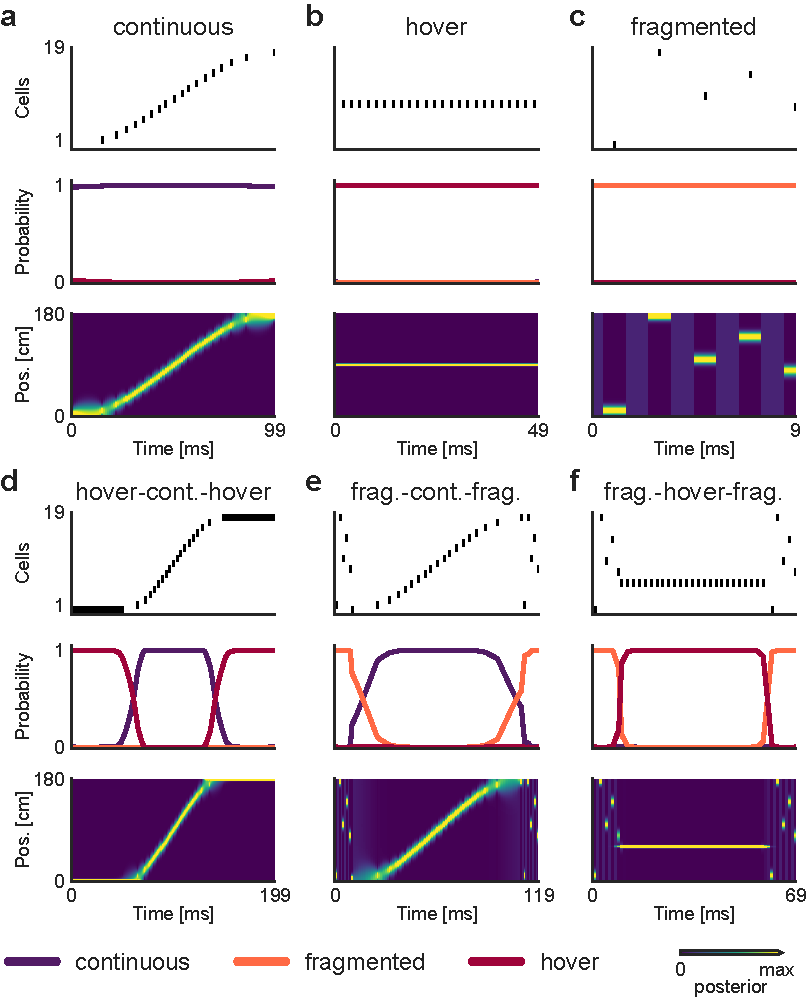
\includegraphics[width=1.0\linewidth]{figures/Figure2.pdf}
\caption{Simulated data used to fit the encoding model. \textbf{a.} Place fields for each simulated neuron are evenly spaced Gaussians with a maximum firing rate of 15 spikes / s. \textbf{b.} Linear position is simulated as a sinusoid to mimic an animal moving back and forth on a linear track. Each neuron spikes according to its place field rate and Poisson distribution.}
\label{fig:computerNo}
\end{figure}

\Blindtext

Figure \ref{fig:computerNo} shows an example of how to insert a column-wide figure. To insert a figure wider than one column, please use the \verb|\begin{figure*}...\end{figure*}| environment. Figures wider than one column should be sized to 11.4 cm or 17.8 cm wide. Use \verb|\begin{SCfigure*}...\end{SCfigure*}| for a wide figure with side captions.

\section*{Discussion}

blablaba \ref{fig:computerNo} 
\blindtext

\subsection*{Blabla} 
\blindtext


blablaba \ref{fig:computerNo}
\blindtext

\begin{acknowledgements}
\blindtext
\end{acknowledgements}

\section*{Bibliography}
\bibliography{zHenriquesLab-Mendeley}

\onecolumn
\newpage

\section*{Materials and Methods}

\subsection*{Filter Derivation}
\begin{enumerate}
\item Use Bayes theorem to define the posterior in terms of a data-derived likelihood and a prior ($ posterior \propto likelihood * prior $)
$$
p(x_{k}, I_{k} \mid y_{1:k}) \propto p(y_{k} \mid x_{k}, I_{k}) * p(x_{k}, I_{k} \mid y_{1:k-1})
$$

\item Use Chapman-Kolmogorov to define prior in terms of previous time step's posterior and state transitions
$$
\begin{align*}
p(x_{k}, I_{k} \mid y_{1:k-1}) &= \sum_{I_{k-1}} \int p(x_{k}, x_{k-1}, I_{k}, I_{k-1} \mid y_{1:k-1}) * dx_{k-1}
\\ &= \sum_{I_{k-1}} \int p(x_{k}, I_{k} \mid x_{k-1}, I_{k-1}, y_{k-1}) * p(x_{k-1}, I_{k-1} \mid y_{1:k-1}) * dx_{k-1}
\\ &= \sum_{I_{k-1}} \int p(x_{k}, I_{k} \mid x_{k-1}, I_{k-1}) * p(x_{k-1}, I_{k-1} \mid y_{1:k-1}) * dx_{k-1}
\\ &= \sum_{I_{k-1}} \int p(x_{k} \mid x_{k-1}, I_{k}, I_{k-1}) * Pr(I_{k} \mid I_{k-1}) * p(x_{k-1}, I_{k-1} \mid y_{1:k-1}) * dx_{k-1}
\end{align*}$$

where:
$p(x_{k-1}, I_{k-1} \mid y_{1:k-1})$ is the previous posterior,
$Pr(I_{k} \mid I_{k-1})$ is the discrete state transition, and $p(x_{k} \mid x_{k-1}, I_{k}, I_{k-1})$ is the continuous state transition

\item Final Filter
$$
p(x_{k}, I_{k} \mid y_{1:k}) \propto p(y_{k} \mid x_{k}, I_{k}) * \sum_{I_{k-1}} \int p(x_{k} \mid x_{k-1}, I_{k}, I_{k-1}) * Pr(I_{k} \mid I_{k-1}) * p(x_{k-1}, I_{k-1} \mid y_{1:k-1}) * dx_{k-1}
$$
\end{enumerate}

\subsection*{Smoother Derivation}

\begin{enumerate}
\item
$$
\begin{align*}
p(x_{k}, I_{k} \mid y_{1:T}) &= \sum_{I_{k+1}} \int p(x_{k}, x_{k+1}, I_{k}, I_{k+1} \mid y_{1:T}) * dx_{k+1}
\\ &= \sum_{I_{k+1}} \int p(x_{k}, I_{k} \mid x_{k+1}, I_{k+1}, y_{1:T}) * p(x_{k+1}, I_{k+1} \mid y_{1:T}) * dx_{k+1}
\\ &= \sum_{I_{k+1}} \int p(x_{k}, I_{k} \mid x_{k+1}, I_{k+1}, y_{1:k}) * p(x_{k+1}, I_{k+1} \mid y_{1:T}) * dx_{k+1}
\\ &= \sum_{I_{k+1}} \int \frac{p(x_{k}, I_{k}, x_{k+1}, I_{k+1} \mid y_{1:k})}{p(x_{k+1}, I_{k+1} \mid y_{1:k})} * p(x_{k+1}, I_{k+1} \mid y_{1:T}) * dx_{k+1}
\\ &= \sum_{I_{k+1}} \int \frac{p(x_{k+1}, I_{k+1} \mid x_{k}, I_{k}, y_{1:k}) * p(x_{k}, I_{k} \mid y_{1:k})}{p(x_{k+1}, I_{k+1} \mid y_{1:k})} * p(x_{k+1}, I_{k+1} \mid y_{1:T}) * dx_{k+1} 
\\ &= \sum_{I_{k+1}} \int \frac{p(x_{k+1}, I_{k+1} \mid x_{k}, I_{k}) * p(x_{k}, I_{k} \mid y_{1:k})}{p(x_{k+1}, I_{k+1} \mid y_{1:k})} * p(x_{k+1}, I_{k+1} \mid y_{1:T}) * dx_{k+1}
\\ &= p(x_{k}, I_{k} \mid y_{1:k}) * \sum_{I_{k+1}} \int \frac{p(x_{k+1}, I_{k+1} \mid x_{k}, I_{k})}{p(x_{k+1}, I_{k+1} \mid y_{1:k})} * p(x_{k+1}, I_{k+1} \mid y_{1:T}) * dx_{k+1} 
\\ &= p(x_{k}, I_{k} \mid y_{1:k}) * \sum_{I_{k+1}} \int \frac{p(x_{k+1} \mid x_{k}, I_{k+1}, I_{k}) * Pr(I_{k+1} \mid I_{k}, x_{k})}{p(x_{k+1}, I_{k+1} \mid y_{1:k})} * p(x_{k+1}, I_{k+1} \mid y_{1:T}) * dx_{k+1}
\end{align*}$$

\item
$$
\begin{align*}
p(x_{k+1}, I_{k+1} \mid y_{1:k}) &= \sum_{I_{k}} \int p(x_{k+1}, I_{k+1}, x_{k}, I_{k} \mid y_{1:k}) * dx_{k}
\\ &= \sum_{I_{k}} \int p(x_{k+1}, I_{k+1} \mid x_{k}, I_{k}, y_{1:k}) * p(x_{k}, I_{k} \mid y_{1:k}) * dx_{k}
\\ &= \sum_{I_{k}} \int p(x_{k+1}, I_{k+1} \mid x_{k}, I_{k}) * p(x_{k}, I_{k} \mid y_{1:k}) * dx_{k}
\\ &= \sum_{I_{k}} \int p(x_{k+1} \mid x_{k}, I_{k+1}, I_{k}) * Pr(I_{k+1} \mid I_{k}) * p(x_{k}, I_{k} \mid y_{1:k}) * dx_{k}
\end{align*}$$

\end{enumerate}

\newpage

%%%%%%%%%%%%%%%%%%%%%%%%%%%%%
% Supplementary Information %
%%%%%%%%%%%%%%%%%%%%%%%%%%%%%
\captionsetup*{format=largeformat}
\section{Something about something} \label{note:Note1} 
\Blindtext

%TC:endignore
%the command above ignores this section for word count

\end{document}
